\documentclass{./../../Latex/teaching_slides}
\usepackage{venndiagram}
\usepackage{tikz}
\usepackage{pgfplots}
\usetikzlibrary{arrows.meta}

\begin{document}

\title{ECON 441 \\ \vspace{0.4em} \normalsize Introduction to Mathematical Economics}
\author{Div Bhagia}
\date{Lecture 1: Preliminaries}

\begin{frame}[noframenumbering, plain]
\maketitle
\end{frame}


\begin{frame}{Today's Topics \& References}
\begin{witemize}
\item Numbers and sets (sections 2.2 and 2.3)
\item Relations and functions (sections 2.4-2.6, page 163)
\item Summation notation (handout)
\item Necessary and sufficient conditions (beginning of 5.1) 
\end{witemize}
\end{frame}

%%%%%%%%%%%%%%%%%%%%%%%% Numbers and Sets
\section{Numbers and Sets}
\begin{frame}{Real-Number System}
\begin{itemize}
\item \textit{Integers}: 
$$...,-3,-2,-1,0,1,2,3,...$$
\item \pause \textit{Fractions}: 
$$ \frac{1}{2}, \frac{3}{5}, -\frac{2}{3}$$
\vspace{0.25em}
\item \pause \textit{Rational numbers}: ratio of integers 
\vspace{0.25em}
\item[] \pause \textit{Are fractions rational numbers? What about integers?}
\end{itemize}
\end{frame}

\begin{frame}{Real-Number System}
\vspace{-0.15em} 
\begin{itemize}
\item \textit{Rational numbers}: ratio of integers 
\item[] \hspace{0.5em} ``terminating or repeating decimal''
\vspace{-0.15em} 
\item[] $$\text{Example. } \frac{1}{3}=0.333, \frac{1}{4}=0.25$$ \\~\\
\vspace{-0.15em} 
\item \pause \textit{Irrational numbers:} cannot be expressed as a ratio of two integers
\item[] \hspace{0.5em} ``nonterminating or nonrepeating decimal'' 
\vspace{-0.15em} 
\item[] $$\text{Example. } \sqrt{2}=1.4142, \pi=3.1415$$ \\~\\
\vspace{-0.15em} 
\item \pause \textit{Real numbers ($\mathbb{R}$): rational and irrational}
\end{itemize}
\end{frame}


\begin{frame}{Sets}
\begin{itemize}
\item A \textit{set} is a collection of distinct objects.
$$ A = \{brownies, icecream, pizza, ramen\} $$
\item $pizza \in A$, $\in$ stands for `is in' \\~\\
%\item \textit{Is $A$ finite? Is it countable?} \\~\\
\item \pause What about sets $B$ and $C$?
$$ B = \{x | x \text{ is a positive integer}\}$$
$$ C = \{x | 1<x<5\}$$
\end{itemize}
\end{frame}

\begin{frame}{Set Relations}
\begin{itemize}
\item[1.] Equivalence ($=$)
$$ A = \{brownies, icecream, pizza, ramen\} $$
$$ B = \{pizza, ramen, icecream, brownies\} $$
$$ A = B $$
\item[2.] \pause Subset ($\subset$)
$$ C = \{pizza, ramen\} $$
$ C \neq A$ but $ C \subset A$. \\ Note: $A \supset C$ is equivalent. \\~\\
\pause \textit{Is $A \subset B$? \pause Yes, but $C$ is a proper subset of A.}
\end{itemize}
\end{frame}

\begin{frame}{Set Relations}
\begin{itemize}
\item[3.] Disjoint sets $$ A = \{brownies, icecream, pizza, ramen\} $$
$$ D = \{salad, fruits\} $$ \\~\\
\item[4.] \pause Neither but still related  $$ A = \{brownies, icecream, pizza, ramen\} $$
$$ E = \{salad, fruits, icecream\} $$
\end{itemize}
\end{frame}

\begin{frame}{Set Relations}
\begin{itemize}
\item $\emptyset$: empty or null set \\~\\
\item \pause What are all possible subsets of $$S = \{a,b,c\}$$
\item[] \pause $\emptyset, \{a\}, \{b\},\{c\}, \{a,b\}, \{b,c\}, \{a,c\}, \{a,b,c\}$  \\~\\
\pause Always $2^n$ subsets. Here $n=3$, so 8 subsets.
\end{itemize}
\end{frame}

\begin{frame}{Set Operations}
\begin{itemize}
\item[1.] \textit{Union:} $A \cup B$, elements in either $A$ \textit{or} $B$
\item[2.] \textit{Intersection:} $A \cap B$, elements in both $A$ \textit{and} $B$ \\~\\
\end{itemize}
Example: 
$$ A = \{brownies, icecream, pizza, ramen\} $$
$$ B = \{salad, fruits, icecream\} $$
$A \cup B = $ \\~\\
$A \cap B = $
\end{frame}

\begin{frame}{Set Operations}
\begin{itemize}
\item[1.] \textit{Union:} $A \cup B$, elements in either $A$ or $B$
\item[2.] \textit{Intersection:} $A \cap B$, elements in both $A$ and $B$ \\~\\
\end{itemize}
What about
$$ A = \{brownies, icecream, pizza, ramen\} $$
$$ B = \{salad, fruits\} $$
$A \cup B = $ \\~\\
$A \cap B = $
\end{frame}

\begin{frame}{Set Operations}
\begin{itemize}
\item[3.] \textit{Complement of $A$}: $\tilde{A}$, `not $A$' \\~\\
\item[] Universal set $U$ (context specific) then: 
$$ \tilde{A}= \{x | x \in U \text{ and } x \not\in A\} $$ \\~\\
Example. $U=\{1,e,f,2\}, A=\{1,2\}$, then $\tilde{A}=\{e,f\}$.
\end{itemize}
\end{frame}

\begin{frame}{Set Operations: Venn Diagrams}
\vspace{1em}
\centering
\begin{venndiagram2sets}[tikzoptions={scale=0.75, thick}]
\end{venndiagram2sets}
\begin{venndiagram2sets}[tikzoptions={scale=0.75, thick}]
\end{venndiagram2sets} \\
\vspace{2.25em}
\begin{venndiagram2sets}[tikzoptions={scale=0.75, thick}]
\end{venndiagram2sets}
\end{frame}

\begin{frame}{Laws of Set Operations}
\begin{itemize}
\item Commutative law
$$ A \cup B = B \cup A \quad \quad  A \cap B = B \cap A$$ \\~\\
\item Distributive law
$$ A \cup (B \cap C) = (A \cup B) \cap (A \cup C) $$
$$ A \cap (B \cup C) = (A \cap B) \cup (A \cap C) $$
\end{itemize}
\end{frame}

\begin{frame}{Distributive law}
\centering
 \fcolorbox{black}{grey}{$A \cup (B \cap C)$} $= (A \cup B) \cap (A \cup C) $ \\~\\
\vskip-0.65em
 \begin{columns}[T]
\begin{column}{0.5\textwidth}
\centering $A$ \\ \vspace{0.5em}
\begin{venndiagram3sets}[tikzoptions={scale=1,very thick}]
\fillA
\end{venndiagram3sets}  	
\end{column}	
\begin{column}{0.5\textwidth}
\centering $B \cap C $ \\ \vspace{0.5em}
\begin{venndiagram3sets}[tikzoptions={scale=1,very thick}]
\fillBCapC
\end{venndiagram3sets}
\end{column}	
\end{columns}
\end{frame}

\begin{frame}{Distributive law}
\centering
$A \cup (B \cap C)=$  \fcolorbox{black}{grey}{$(A \cup B) \cap (A \cup C) $} \\~\\
\vskip-0.65em
\begin{columns}[T]
\begin{column}{0.5\textwidth}
\centering $A \cup B$ \\ \vspace{0.5em}
\begin{venndiagram3sets}[tikzoptions={scale=1,very thick}]
\fillA \fillB
\end{venndiagram3sets}  	
\end{column}	
\begin{column}{0.5\textwidth}
\centering $A \cup C$ \\ \vspace{0.5em}
\begin{venndiagram3sets}[tikzoptions={scale=1,very thick}]
\fillA \fillC
\end{venndiagram3sets}
\end{column}	
\end{columns}
\end{frame}

\begin{frame}{Ordered Sets}
\begin{itemize}
\item We said order does not matter for sets
\item But we can have ordered sets where 
$$ (a,b) \neq (b,a) \text{ unless } a=b$$
\item Ordered pairs, triples,... \\~\\
\end{itemize}
Example. $(age, weight)$, $(22,120)$ different from $(120,22)$
\end{frame}

% \begin{frame}{Cartesian Plane}
% \centering
% \vfill
% \begin{tikzpicture}
% \begin{axis}[
%   axis lines=middle,
%   axis line style={Stealth-Stealth,very thick},
%   xmin=-4.5,xmax=4.5,ymin=-4.5,ymax=4.5,
%   xtick distance=1,
%   ytick distance=1,
%   xlabel=$x$,
%   ylabel=$y$,
%   %title={Wonderful plot},
%   grid=major,
%   grid style={thin,densely dotted,black!20}]
% %\addplot [Latex-Latex,domain=-5:3,samples=2] {x*2/3} node[right]{$a$};
% \end{axis}
% \end{tikzpicture}
% \end{frame}

\begin{frame}{Cartesian Product}
$$ A = \{1,2\} \quad B = \{3,4\} $$ \\~\\
Cartesian Product: set of all possible ordered pairs
$$ A \times B = \{ (1,3), (1,4), (2,3), (2,4) \} $$
\end{frame}

\begin{frame}{Cartesian Plane}
\vspace{-1em}
$$ \mathbb{R}^2 =  \{(x,y) | x \in \mathbb{R}, y \in \mathbb{R}\} $$
\centering
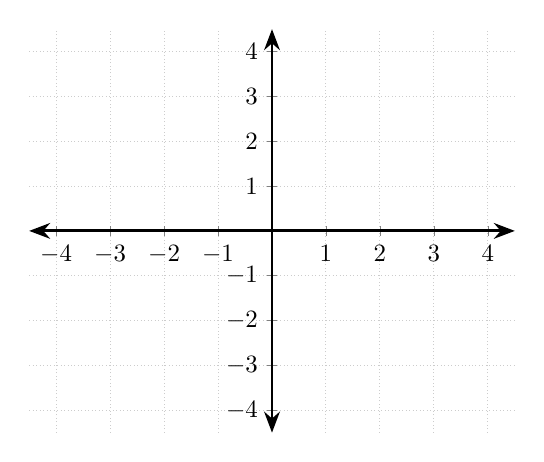
\begin{tikzpicture}[scale=0.9]
\begin{axis}[
  axis lines=middle,
  axis line style={Stealth-Stealth,very thick},
  xmin=-4.5,xmax=4.5,ymin=-4.5,ymax=4.5,
  xtick distance=1,
  ytick distance=1,
  %xlabel=$x$,
  %ylabel=$y$,
  %title={Wonderful plot},
  grid=major,
  grid style={thin,densely dotted,black!20}]
%\addplot [Latex-Latex,domain=-5:3,samples=2] {x*2/3} node[right]{$a$};
\end{axis}
\end{tikzpicture} \\~\\
\hspace{-3cm} Can have $ \mathbb{R}^3, \mathbb{R}^4,...,\mathbb{R}^n $
\end{frame}

%%%%%%%%%%%%%%%%%%%%%%%% Relations and Functions
\section{Relations and Functions}

\begin{frame}{Relations}
Relation: subset of the Cartesian product \\~\\
Example. $\{(x,y) | y \leq x \} $

\centering
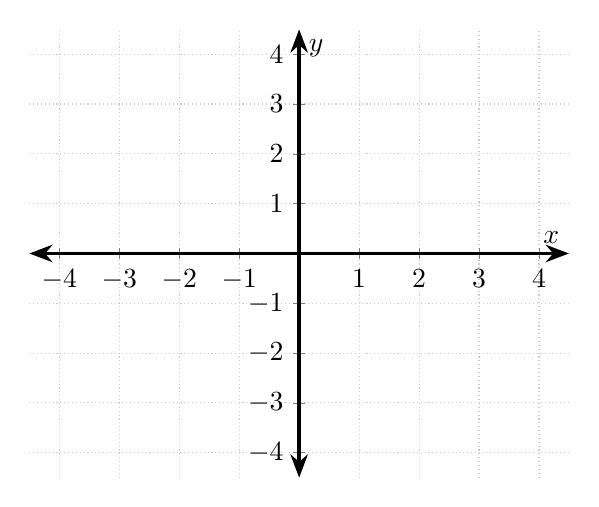
\begin{tikzpicture}
\begin{axis}[
  axis lines=middle,
  axis line style={Stealth-Stealth,very thick},
  xmin=-4.5,xmax=4.5,ymin=-4.5,ymax=4.5,
  xtick distance=1,
  ytick distance=1,
  xlabel=$x$,
  ylabel=$y$,
  %title={Wonderful plot},
  grid=major,
  grid style={thin,densely dotted,black!20}]
%\addplot [Latex-Latex,domain=-5:3,samples=2] {x*2/3} node[right]{$a$};
\end{axis}
\end{tikzpicture}

\end{frame}

\begin{frame}{Functions}
 Function: a relation where for each $x$ there is a unique $y$  
$$ f: X \rightarrow Y, \quad y = f(x) $$ \\~\\
Examples. $y = x, y=x^2, y=2x+3 $ \\~\\

$X:$ domain, $Y:$ codomain, $f(X):$ range \\~\\

Most functions we will encounter, $f: \mathbb{R}^k \rightarrow \mathbb{R}$

\end{frame}


\begin{frame}{Functions}
Let's say,
$$ f: X \rightarrow \mathbb{R}, \quad y = 3x-5 $$ \\~\\
where $ X = \{2,3,4\} $. \\~\\
What is the range?

\end{frame}

\begin{frame}{Cost Function}
Consider the total cost $C$ of producing hats $Q$,
$$ C = f(Q) $$
\begin{itemize}
\item Should I be able to produce 10 hats and 5 hats at the same cost? \\~\\
\item Possible to produce 5 hats for \$20 and \$25?
\end{itemize}
\end{frame}

\begin{frame}{By the way}
Consider the total cost $C$ of producing hats $Q$,
$$ C = f(Q) = 2Q + 5 $$
\vspace{0.3em}

What is the cost of producing 1 hat? \\~\\
What is the cost of producing 2 hats? \\~\\
How many hats can I produce for \$25?
\end{frame}

\begin{frame}{Types of Functions}

\begin{itemize}
\item Constant: $y = f(x) = 5$ \\~\\
\item Polynomial of degree $n$ 
\begin{itemize}
\item[] $n=0$, constant
\item[] $n=1$, linear
\item[] $n=2$, quadratic
\item[] $n=3$, cubic
\item[] ...
\end{itemize}
\item Rational function: ratio of two polynomial functions:
$$ y = \frac{a}{x} $$
\end{itemize}
\end{frame}

\begin{frame}{Function of More than One Variables}
Functions can be of two variables:
$$ z=g(x,y) $$
Or three, or four,..., or $n$
\end{frame}


\begin{frame}{Monotonic functions}
	Strictly increasing function:
$$ x_{1}>x_{2} \rightarrow f\left(x_{1}\right)>f\left(x_{2}\right) $$
Strictly decreasing function:
$$ x_{1}>x_{2} \rightarrow f\left(x_{1}\right)<f\left(x_{2}\right) $$
Increasing function:
$$ x_{1}>x_{2} \rightarrow f\left(x_{1}\right)\geq f\left(x_{2}\right) $$
Decreasing function:
$$ x_{1}>x_{2} \rightarrow f\left(x_{1}\right)\leq f\left(x_{2}\right) $$
\end{frame}

\begin{frame}{Inverse of a function}
Function $y=f(X)$ has an inverse if it is a one-to-one mapping, i.e. each value of $y$ is associated with a unique value of $x$. \\~\\
Inverse function $$x=f^{-1}(y)$$ returns the value corresponding value of $x$ for each $y$. \\~\\
One-to-one mapping unique to strictly monotonic functions
\end{frame}

\begin{frame}{Inverse of a function}
Example: Find the inverse of $y = f(x) = 3x-2$. 
\end{frame}

\begin{frame}{By the way}
What is $x \times x$? \\~\\
What is $x^2 \times x$? \\~\\
What is $x^2 \times x^2$? \\~\\
More generally, $x^n \times x^m = x^{m+n}$
\end{frame}

%%%%%%%%%%%%%%%%%%%%%%%% Summation Notation
\section{Summation Notation}

\begin{frame}[t]{Summation Notation}

$$ \sum_{i=1}^N x_i = x_1 + x_2 + ... + x_N $$

\vspace{1em}
\underline{\textit{Example:}} \\
\vspace{0.5em}
$x = \{2,9,6,8,11,14\}$ \\
\vspace{1em}
$\sum_{i=1}^{4} x_i = x_1 + x_2 + x_3 + x_4 = 2+9+6+8=25$ 
\end{frame}

%%%%%%%%%%%%%%%%%%%%
\begin{frame}{Summation Notation}
Another way of using a summation sign is to write $$\sum_{x \in A} x $$
which refers to summing up all elements in $A$. \\~\\
To sum up $x$ for all possible values $x$, we can simply write $$\sum_x x$$
\end{frame}


\begin{frame}{Things you CAN do}
\begin{enumerate}
\item Pull constants out of or into the summation sign.
$$ \sum_{i=1}^N b x_i = b \sum_{i=1}^N x_i  $$
\end{enumerate}
\end{frame}

\begin{frame}{Things you CAN do}
\begin{enumerate}
\item[2.] Split apart (or combine) sums (addition) or differences (subtraction)
$$ \sum_{i=1}^N (b x_i + c y_i) = b \sum_{i=1}^N x_i  + c \sum_{i=1}^N y_i $$
\end{enumerate}
\end{frame}

\begin{frame}{Things you CAN do}
\begin{enumerate}
\item[3.] Multiply through constants by the number of terms in the summation
$$ \sum_{i=1}^N (a+b x_i)= aN + b \sum_{i=1}^N x_i  $$
\end{enumerate}
\end{frame}

\begin{frame}{Things you CANNOT do}
\begin{enumerate}
\item Split apart (or combine) products (multiplication) or quotients (division).
$$ \sum_{i=1}^N x_i y_i \neq  \sum_{i=1}^N x_i \times \sum_{i=1}^N y_i   $$
\end{enumerate}
\end{frame}

\begin{frame}{Things you CANNOT do}
\begin{enumerate}
\item[2.] Move the exponent out of or into the summation.
$$ \sum_{i=1}^N x_i^a \neq  \left(\sum_{i=1}^N x_i\right)^a $$
\end{enumerate}
\end{frame}

%%%%%%%%%%%%%%%%%%%%%%%% Necessary and Sufficient Conditions
\section{Necessary and Sufficient Conditions}
\begin{frame}{Necessary vs. Sufficient Conditions}
$q$ is a necessary condition for $p$ if:
$$ p \implies q $$ 
\vspace{1em}

\pause
$p$:  I ate tofu for dinner  \\~\\
$q$:  My dinner had protein
\end{frame}

\begin{frame}{Necessary vs. Sufficient Conditions}
$q$ is a sufficient condition for $p$ if:
$$ p \impliedby q $$ 
\vspace{1em}

\pause
$p$:  A number is even \\~\\
$q$:  A number is divisible by 4
\end{frame}

\begin{frame}{Necessary vs. Sufficient Conditions}
$q$ is both necessary and sufficient for $p$
$$ p \iff q $$ 
\vspace{1em}

\pause
$p$:  A number is even \\~\\
$q$:  A number is divisible by 2
\end{frame}

\begin{frame}{Necessary vs. Sufficient Conditions}
\vspace{1em}


$p$:  It is a holiday  \\~\\
$q$:  It is Thanksgiving
\end{frame}

\begin{frame}{Necessary vs. Sufficient Conditions}
\vspace{1em}


$p$: The car is out of gas  \\~\\
$q$: The car isn't starting
\end{frame}

\begin{frame}{Necessary vs. Sufficient Conditions}
\vspace{1em}
$p$:  A geometric figure has four sides  \\~\\
$q$:  It is a rectangle
\end{frame}

\begin{frame}{Homework Questions}
\begin{witemize}
  \item Exercise 2.3: 1, 2
  \item Exercise 2.4: 5, 7, 8
  \item Exercise 2.5: 1 (For each part, find the inverse of the function too.)
  \item Exercise 4.2: 6, 8
  \item Exercise 5.1: 1
\end{witemize}
\end{frame}


\end{document}